\documentclass[11pt, sigconf]{acmart}
\begin{document}

%%
%% The "title" command has an optional parameter,
%% allowing the author to define a "short title" to be used in page headers.
\title{CS2309 Research Proposal: L4}

%%
%% The "author" command and its associated commands are used to define
%% the authors and their affiliations.
%% Of note is the shared affiliation of the first two authors, and the
%% "authornote" and "authornotemark" commands
%% used to denote shared contribution to the research.
\author{Yee Jian Tan}
\email{yeejian.tan@u.nus.edu}
\orcid{0000-0002-5725-9633}
\affiliation{%
  \institution{National University of Singapore}
  \streetaddress{22 College Avenue East}
  \country{Singapore}
  \postcode{138595}
}

\begin{abstract}
  The L4 language is a domain-specific language (DSL) designed to encode legal
  texts. On top of that, it is designed to analyze and reason with legal texts
  via SMT (and ASP) solvers. However, since it is a language still in
  development, there has not been mathematical verification of its completeness
  and consistency as a law DSL. This research proposal aims to sketch a plan
  using logic, automata and type theory as directions to investigate and
  formally verify this newly-formulated language.

\end{abstract}

\begin{CCSXML}
<ccs2012>
   <concept>
       <concept_id>10011007.10011006.10011008.10011009.10011015</concept_id>
       <concept_desc>Software and its engineering~Constraint and logic languages</concept_desc>
       <concept_significance>300</concept_significance>
       </concept>
   <concept>
       <concept_id>10011007.10011006.10011050.10011017</concept_id>
       <concept_desc>Software and its engineering~Domain specific languages</concept_desc>
       <concept_significance>500</concept_significance>
       </concept>
   <concept>
       <concept_id>10003752.10003790.10002990</concept_id>
       <concept_desc>Theory of computation~Logic and verification</concept_desc>
       <concept_significance>500</concept_significance>
       </concept>
   <concept>
       <concept_id>10003752.10003766</concept_id>
       <concept_desc>Theory of computation~Formal languages and automata theory</concept_desc>
       <concept_significance>300</concept_significance>
       </concept>
   <concept>
       <concept_id>10010405.10010455.10010458</concept_id>
       <concept_desc>Applied computing~Law</concept_desc>
       <concept_significance>500</concept_significance>
       </concept>
 </ccs2012>
\end{CCSXML}

\ccsdesc[300]{Software and its engineering~Constraint and logic languages}
\ccsdesc[500]{Software and its engineering~Domain specific languages}
\ccsdesc[500]{Theory of computation~Logic and verification}
\ccsdesc[300]{Theory of computation~Formal languages and automata theory}
\ccsdesc[500]{Applied computing~Law}

%%
%% Keywords. The author(s) should pick words that accurately describe
%% the work being presented. Separate the keywords with commas.
\keywords{computational law, type theory, temporal logic}

%% A "teaser" image appears between the author and affiliation
%% information and the body of the document, and typically spans the
%% page.
\begin{teaserfigure}
  \fbox{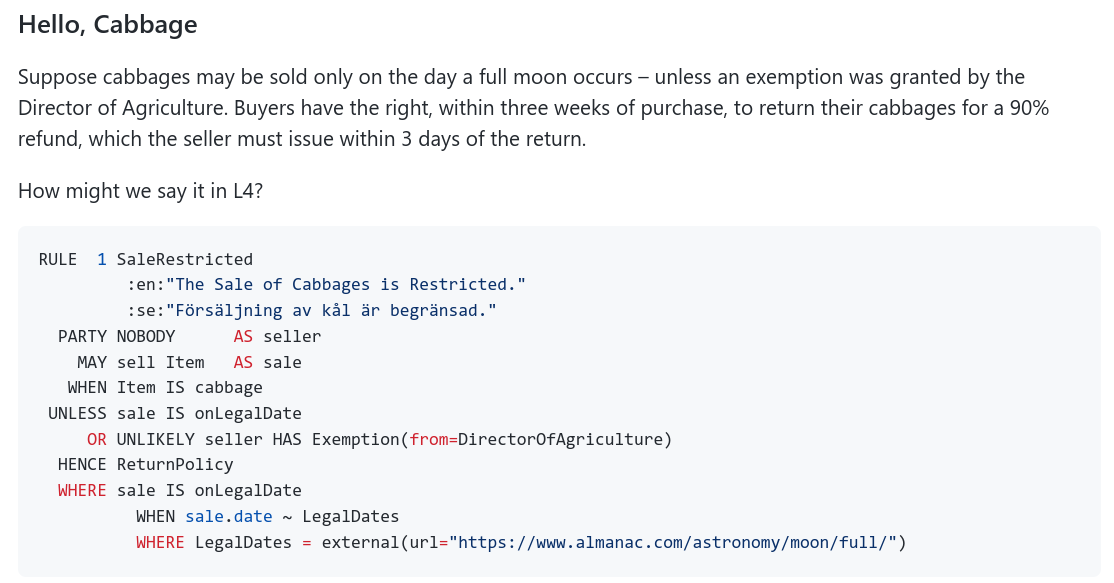
\includegraphics[width=\textwidth]{cabbage}}
  \caption{The L4 Language. Taken from \url{https://github.com/smucclaw/dsl/} on
    13 November 2021.}
  \label{fig:teaser}
\end{teaserfigure}
%%
%% This command processes the author and affiliation and title
%% information and builds the first part of the formatted document.
\maketitle
\section{Introduction}
\label{sec:intro}
This research proposal is inspired by, and builds on the work of SMU Center of
Computational Law (CCLAW) \cite{smucclaw, singapore_management_university_2021}.

Legal documents are essentially a series of logical rules. They state conditions
to be fulfilled with their consequences and alternates, no different from a
typical \emph{if-then-else} clause in programming. Formulating law into computer
programs have been an active area of research, and multiple approaches have been
taken. In particular, the SMU CCLAW has decided to write a Domain Specific
Language (DSL), called L4, which encodes law text and provides a way to
``compile'' into natural language. More importantly, this DSL should be designed
for analysis and verification in mind. Are there any conditions which is
impossible to fulfill? Are there contradicting conditions which make certain
rules ambiguous or redundant? To answer these questions, our DSL should allow
analysis from they way it is designed.

L4, the language by SMU CCLAW, can allow different ways of analysis, including
Satisfiable Modulo Theory (SMT) and Answer Set Programming (ASP). As a DSL to
encode legal texts, we have to ensure that the language is complete and
consistent. Complete as in it can encode any legal truth as stated in the
documents, consistent as in the elimination rules of the semantics of the L4
language conforms to a subset of the natural deduction and hence is not
self-contradictory.

\section{Problem and Proposal}
\label{sec:problem}
We ask the question: \textbf{is the L4 language complete and consistent?}
Although the authors should have paid sufficient attention to this regard, it is
nonetheless paramount that the completeness and consistency of the system be
\textbf{proven formally and mathematically}, especially for a domain as
important as legal formalization. As of the time of writing, there are no such
proofs to be found in the papers as provided in their Github repository
\cite{smucclaw}. I propose to answer this problem in 2 methods: first by
exploring related \textbf{automata and logical systems }that are similar to that
of law, secondly proving the inherent completeness and consistency of the system
by the angle of \textbf{type theory}.

\subsection{Automata and logical systems}
\label{subsec:automata}

In the approach to look at existing logic and automaton, we explore what are the
logic systems in use for computational law, most likely systems such as Linear
Temporal Logic, Buchi (Temporal) Automaton, as well as deontic logic and
defeasible reasoning, which are prevalent in law (\cite{sep-logic-deontic},
\cite{sep-reasoning-defeasible}). Understanding how these theories fit with the
L4 language would enable an inspection in the capabilities and differences
between the logic of L4 and any selected system, and any significant differences
or contradictions would signify a need to change the specifications of the L4
language.

\subsection{Type Theory}
\label{subsec:tt}
The L4 language uses the concept of classes (or types), so it is natural to
analyze this hierachy of type-induced propositions in the language. Type Theory
refers to the study of typed lambda calculus systems such as Martin-Lof Type
Theory and Homotopy Type Theory, and their correspondence to mathematical logic.
The use of types in languages inherently gets its ``proof strength'' from the
corresponding logical systems \cite{sep-type-theory}. Existing logical systems
in proof assistants such as Coq are not designed for the \emph{temporal} way of
reasoning in law, where an action done in different time can lead to different
consequences. There are existing systems which aim to bring temporal logic to
Coq, however implementations differ and it is not yet standardized
\cite{notbad4u_2019, gmalecha_2015}. Another system of importance is Temporal
Type Theory, which is known to already embed Linear and Metric Temporal Logic
\cite{schultz2017temporal}, fits the use case of L4 well.

\section{Related works}
\label{sec:related}
The Catala language \cite{merigoux2021catala} is a ``programming language for
law'', one of the most prominent DSL for law. The compilation of Catala is
verified by the \emph{F*} theorem prover. Catala has a multi-step compilation
process, first translating from the concrete syntax to a desugared \emph{scope
  language}, which is in turn translated into a lambda calculus-like
\emph{default calculus}, before compiling to a programming language such as
OCaml that has runtime exceptions \cite{merigoux2021catala}.

The approach to code legal reasoning with type theory so the facts can be proven
mathematically is not new. LogiKEy workbench \cite{logikey} uses the Isabelle
interative proof assistant to code and prove legal rules, differing from the
approach taken by L4 to use SMT and Answer Set Programming (ASP) solvers to
automatically prove theorems \cite{smucclaw}. Even so, the integration between a
DSL for law and a proof assistant would be worth investigating, and is important
to our research since proving facts about legal texts are a main part of what
lawyers do.

As for logic, deontic logic and defeasible reasoning are two important starting
points to explore the completeness of the L4 system \cite{smucclaw}. Deontic
logic is concerned about notions such as ``the least one can do'',
``obligatory'', ``permissible'' and other similar concepts, which often occur in
law \cite{sep-logic-deontic}. Deontic logic is emphasized in systems such as
Symboleo \cite{Symboleo} and the NAI Suite
\cite{libal_steen_nai_suite_draft_reason_legal_texts_jurix_2019}. On the other
hand, defeasible reasoning is about reasonings that are ``rationally compelling
but not deductively valid'', ie., when the premises are true but the derived
conclusion is false. A combination of both deontic logic and defeasible
reasoning forms the base of the Turnip system \cite{governatori1,
  Governatori2021UnravelLR}, developed by Governatori and colleagues.

\section{Methodology}
\label{sec:method}
To explore completeness of the existing L4 system, we will investigate by
encoding a small piece of law or legal contract in L4 to explore the
completeness requirements. Then by exploring existing systems as well and
considering both deontic logic and defeasible reasoning, another survey on
temporal logic and automata to match these features would be the end goal of the
completeness investigation.

The type theory approach has two non-overlapping directions of investigation:
one to explore extending L4's type system to temporal type theory
\cite{schultz2017temporal}. Then it will strengthen the L4 language, such that
it is possible to prove theorems during the encoding of law into L4. However,
this requires care as L4 currently allows users to define their own types, and
self-define types might lead to significant overhead in the SMT and ASP solvers
due to these unintended types-as-propostitions. Another approach would be to use
a theorem prover such as Coq to prove the consistency of the axiomatic system
and elimination rules of L4. This is a requirement before L4 can be more than
merely an encoding of law like a controlled natural language, like an
intermediate representation for SMT and ASP solvers to work on.

\section{Conclusion}
\label{sec:conclusion}

The task to prove the completeness and consistency of the L4 language can be
challenging due to its open-endedness, but many related works already reached
varying levels of success in formalizing law. While their logical systems can be
used as a reference point, L4 is unique in its design to use SMT and ASP solvers
from the start. In this case, the type theory approach is an important
complementary way to show these important properties of this language,
especially via the promising Temporal Type Theory.

\bibliographystyle{ACM-Reference-Format}
\bibliography{references}
\end{document}
